% ============================================================
% Dimension-4 SQIsign at Round-3 Parameters (W05, SECENG-1997)
%
% One source file.  Every number in a table or figure is generated from
% the repository's documents by figures/*.py (`make figures`, see
% FIGURES.md); every number in the prose carries a `% source:` comment.
% Paste main_standalone.tex (bundled by figures/bundle.py) and refs.bib
% into Overleaf.
% ============================================================
\documentclass[11pt]{article}
\usepackage{amsmath,amssymb}
\usepackage[utf8]{inputenc}
\usepackage{hyperref}
\usepackage{enumitem}
\usepackage[margin=1in]{geometry}
\usepackage{microtype}
\usepackage{booktabs}
\usepackage{threeparttable}
\usepackage{xcolor}
\usepackage{tikz}
\usetikzlibrary{arrows.meta,positioning,calc,decorations.pathreplacing}
\usepackage{pgfplots}
\pgfplotsset{compat=1.18}
\usepackage{pgfplotstable}
\usepackage{placeins}
\usepackage{float}

\newcommand{\Fp}{\mathbb{F}_p}
\newcommand{\Fpq}{\mathbb{F}_{p^2}}
\newcommand{\Ecom}{E_{\mathrm{com}}}
\newcommand{\Echl}{E_{\mathrm{chl}}}
\newcommand{\Eaux}{E_{\mathrm{aux}}}
\newcommand{\Epk}{E_{\mathrm{pk}}}
\newcommand{\sP}{strong-PRISM}
\newcommand{\ECL}{ECLIPSE}

% One accent colour per implementation; the same values as figures/common.py.
\definecolor{crefc}{HTML}{4C6A92}    % the C reference, broadwell build
\definecolor{rsdimtwo}{HTML}{8FB3DA} % this crate, dimension 2
\definecolor{rsdimfour}{HTML}{2A9D8F}% this crate, dimension 4 (compact)
\definecolor{rtwoc}{HTML}{D98E2B}    % the round-2 crate
\definecolor{neutralc}{HTML}{6B6B6B}
\definecolor{lightc}{HTML}{BFBFBF}

\pgfplotsset{
  paperplot/.style={
    tick label style={font=\footnotesize},
    label style={font=\footnotesize},
    legend style={font=\footnotesize, draw=none, fill=none},
    axis lines*=left,
  },
}
\tikzset{
  curve/.style={font=\normalsize, minimum width=1.1cm, minimum height=0.55cm,
    inner sep=2pt},
  deg/.style={font=\scriptsize, text=neutralc},
  same/.style={decorate, decoration={brace, amplitude=3pt}, lightc, thin},
  panel/.style={font=\footnotesize, align=center},
  >=Stealth}

% The numbers the prose and captions quote, generated from paper-dim4/BENCH.md and
% docs/COMPACT_R3.md by figures/values.py.
% generated by figures/values.py; do not edit
\newcommand{\EmbedI}{174}
\newcommand{\TorsionRI}{89}
\newcommand{\HalfStepsI}{87}
\newcommand{\LogTwoPI}{325.58}
\newcommand{\PredSigI}{142}
\newcommand{\PredSigAllI}{154}
\newcommand{\SpecSigI}{200}
\newcommand{\LambdaI}{128}
\newcommand{\ExpectedSamplesI}{241}
\newcommand{\ExpectedTestsI}{60}
\newcommand{\ExpectedSamplesOddI}{121}
\newcommand{\EmbedIII}{264}
\newcommand{\TorsionRIII}{134}
\newcommand{\HalfStepsIII}{132}
\newcommand{\LogTwoPIII}{504.75}
\newcommand{\PredSigIII}{214}
\newcommand{\PredSigAllIII}{231}
\newcommand{\SpecSigIII}{306}
\newcommand{\LambdaIII}{192}
\newcommand{\ExpectedSamplesIII}{366}
\newcommand{\ExpectedTestsIII}{91}
\newcommand{\ExpectedSamplesOddIII}{183}
\newcommand{\EmbedV}{346}
\newcommand{\TorsionRV}{175}
\newcommand{\HalfStepsV}{173}
\newcommand{\LogTwoPV}{668.09}
\newcommand{\PredSigV}{280}
\newcommand{\PredSigAllV}{302}
\newcommand{\SpecSigV}{406}
\newcommand{\LambdaV}{256}
\newcommand{\ExpectedSamplesV}{480}
\newcommand{\ExpectedTestsV}{120}
\newcommand{\ExpectedSamplesOddV}{240}
\newcommand{\PredPkI}{84}
\newcommand{\PredPkIII}{130}
\newcommand{\PredPkV}{170}
\newcommand{\PkStdI}{83}
\newcommand{\SigStdI}{200}
\newcommand{\ComboStdI}{283}
\newcommand{\SigCompI}{176}
\newcommand{\PkRtwoStdI}{65}
\newcommand{\SigRtwoStdI}{148}
\newcommand{\PkStdIII}{129}
\newcommand{\SigStdIII}{306}
\newcommand{\ComboStdIII}{435}
\newcommand{\SigCompIII}{269}
\newcommand{\PkRtwoStdIII}{97}
\newcommand{\SigRtwoStdIII}{224}
\newcommand{\PkStdV}{169}
\newcommand{\SigStdV}{406}
\newcommand{\ComboStdV}{575}
\newcommand{\SigCompV}{353}
\newcommand{\PkRtwoStdV}{129}
\newcommand{\SigRtwoStdV}{292}
\newcommand{\PkCompactI}{84}
\newcommand{\SigCompactI}{142}
\newcommand{\ComboCompactI}{226}
\newcommand{\PkRtwoCompactI}{64}
\newcommand{\SigRtwoCompactI}{108}
\newcommand{\ComboRtwoCompactI}{172}
\newcommand{\SigSavingPct}{29}
\newcommand{\VerStdI}{12.2}
\newcommand{\VerCompI}{14.4}
\newcommand{\SignStdI}{113.5}
\newcommand{\KeygenStdI}{39.0}
\newcommand{\VerCrefI}{11.3}
\newcommand{\SignCrefI}{101.4}
\newcommand{\KeygenCrefI}{35.5}
\newcommand{\VerRtwoStdI}{13.6}
\newcommand{\SignRtwoStdI}{429.3}
\newcommand{\KeygenRtwoStdI}{175.8}
\newcommand{\VerCrefRtwoI}{5.3}
\newcommand{\SignCrefRtwoI}{112.4}
\newcommand{\KeygenCrefRtwoI}{48.4}
\newcommand{\VerStdOverCrefI}{1.08}
\newcommand{\KeygenStdOverCrefI}{1.10}
\newcommand{\SignStdOverCrefI}{1.12}
\newcommand{\VerStdIII}{32.7}
\newcommand{\VerCompIII}{35.9}
\newcommand{\SignStdIII}{448.1}
\newcommand{\KeygenStdIII}{137.8}
\newcommand{\VerCrefIII}{28.7}
\newcommand{\SignCrefIII}{371.0}
\newcommand{\KeygenCrefIII}{111.4}
\newcommand{\VerRtwoStdIII}{38.2}
\newcommand{\SignRtwoStdIII}{1653.7}
\newcommand{\KeygenRtwoStdIII}{412.2}
\newcommand{\VerCrefRtwoIII}{17.0}
\newcommand{\SignCrefRtwoIII}{314.4}
\newcommand{\KeygenCrefRtwoIII}{136.9}
\newcommand{\VerStdOverCrefIII}{1.14}
\newcommand{\KeygenStdOverCrefIII}{1.24}
\newcommand{\SignStdOverCrefIII}{1.21}
\newcommand{\VerStdV}{83.0}
\newcommand{\VerCompV}{96.7}
\newcommand{\SignStdV}{922.6}
\newcommand{\KeygenStdV}{280.1}
\newcommand{\VerCrefV}{79.8}
\newcommand{\SignCrefV}{780.6}
\newcommand{\KeygenCrefV}{241.5}
\newcommand{\VerRtwoStdV}{77.1}
\newcommand{\SignRtwoStdV}{3036.1}
\newcommand{\KeygenRtwoStdV}{1169.8}
\newcommand{\VerCrefRtwoV}{32.6}
\newcommand{\SignCrefRtwoV}{527.4}
\newcommand{\KeygenCrefRtwoV}{210.6}
\newcommand{\VerStdOverCrefV}{1.04}
\newcommand{\KeygenStdOverCrefV}{1.16}
\newcommand{\SignStdOverCrefV}{1.18}
\newcommand{\VerCompactI}{120.3}
\newcommand{\VerMultI}{9.9}
\newcommand{\VerMultCrefI}{10.6}
\newcommand{\SignCompactI}{336.6}
\newcommand{\SignMultI}{3.0}
\newcommand{\SignCompactMeanI}{546.2}
\newcommand{\SignCompactMinI}{49.8}
\newcommand{\SignCompactMaxI}{3712.3}
\newcommand{\KeygenCompactI}{41.7}
\newcommand{\KeygenMultI}{1.07}
\newcommand{\VerRtwoCompactI}{108.6}
\newcommand{\VerRtwoMultI}{8.0}
\newcommand{\SignRtwoCompactI}{204.6}
\newcommand{\KeygenRtwoCompactI}{173.8}
\newcommand{\VerCompOverStdPct}{18}
\newcommand{\MsVerStdI}{4.4}
\newcommand{\MsVerCompactI}{43.0}
\newcommand{\MsSignStdI}{40.5}
\newcommand{\MsSignCompactI}{120.2}
\newcommand{\LoopSignatures}{100}
\newcommand{\LoopSamplesMean}{114}
\newcommand{\LoopSamplesMedian}{68}
\newcommand{\LoopSamplesMin}{1}
\newcommand{\LoopSamplesMax}{835}
\newcommand{\LoopTestsMean}{57}
\newcommand{\PeakHeapKiB}{1674}
\newcommand{\PeakHeapMiB}{1.64}
\newcommand{\MachineXeon}{Intel Xeon CPU @ 2.80GHz (8 vCPUs, 31 GiB)}
\newcommand{\XeonGHz}{2.80}
\newcommand{\MFourAvailable}{0}


\title{Dimension-4 SQIsign at Round-3 Parameters:\\
Sizes and Costs of the Compact Format}
\author{Dustin Ray, Anchorage Digital}
\date{September 2026}

\begin{document}
\pagestyle{myheadings}
\markright{Dimension-4 SQIsign at round-3 parameters}
\maketitle

\begin{abstract}
% No citations: ePrint abstracts do not allow them.
% source: paper-dim4/BENCH.md, session 2026-09-26 (sizes table; verify rows);
% docs/COMPACT_R3.md Section 1.
SQIsign holds the smallest known combination among post-quantum
signatures, and its dimension-2 signature
carries an auxiliary curve whose only role is to make the response
computable in dimension 2.  SQIsignHD's dimension-4 response has no such
curve.  We take that construction to the round-3 SQIsign primes, which
replaced the round-2 primes in September 2026 after the attacks of
Wesolowski and others, on our Rust port of the SQIsign reference code, and
measure it in one session next to the reference's own assembly build.  At
NIST level~I the dimension-4 signature is \SigCompactI{} bytes against
\SigStdI{} for the specification's format, with an \PkCompactI-byte public
key: \ComboCompactI{} bytes for key and signature together, the smallest
level-I combination we are aware of, among isogeny schemes and
post-quantum signatures alike, at parameters that stand after those
attacks.  The price is verification: the dimension-4 verifier costs
\VerMultI{} times the dimension-2 verifier of the same code
(\VerCompactI{} against \VerStdI{} megacycles).  The dimension-4
parameters published with SQIsignHD are for its authors' own primes; we
derive them for the round-3 primes, state which choices are SQIsignHD's
and which are ours, and report what was built and measured.
\end{abstract}

% ------------------------------------------------------------------------
\section{Introduction}
\label{sec:intro}

SQIsign is a signature scheme whose public key is an elliptic curve and
whose signature describes a path of curves.  Its first version signed in
seconds and verified fast, with the smallest signatures of any post-quantum
proposal, at the price of a signer built on the KLPT algorithm for finding
paths in the quaternion algebra of the curve~\cite{DKLPW20}.

In 2022 three groups broke the SIDH key exchange by showing how an isogeny
between two elliptic curves can be recovered from its action on a few
points, by embedding it in an isogeny of a higher-dimensional abelian
variety~\cite{CD23,MMPPW23,Rob23}.  The embedding is Kani's~\cite{Kan97}.
What was a weapon against SIDH became a tool for SQIsign: the signer no
longer needs a path of smooth degree, because any isogeny of known degree
can be handed to the verifier through its action on points and rebuilt in
a higher dimension.

SQIsignHD did this in dimension~4~\cite{DLRW24}.  Its signer is fast and
its signature is small, and the whole cost moved to the verifier, which
computes a chain of dimension-4 isogenies.  Its authors released a C
signer and a SageMath verifier~\cite{SQISignHDlib}.  SQIsign2D-West brought
the response back to dimension~2~\cite{BDDF24}: one more isogeny, the
auxiliary one, is computed by the signer so that the verifier's chain
runs on a product of two elliptic curves.  Verification became fast again,
the signature grew by the auxiliary curve, and this design is the round-2
and the round-3 SQIsign submission to NIST~\cite{SQISignV2,SQISignV3}.

In 2026 Wesolowski gave an algorithm for the supersingular isogeny problem
in time and memory $p^{1/3+o(1)}$~\cite{Wes26}.  The round-3 submission of
September 2026 answered with larger primes,
$3 \cdot 2^{324} - 1$, $27 \cdot 2^{500} - 1$ and $17 \cdot 2^{664} - 1$
at levels I, III and V~\cite{SQISignV3}.
% source: README.md first paragraph; docs/COMPACT_R3.md Section 1 table.

This paper takes SQIsignHD's dimension-4 response to those primes.  We
already had a Rust implementation of SQIsign, sqisign-rs, with the round-3
dimension-2 signer and verifier reproducing the reference's known-answer
vectors byte for byte~\cite{SqisignRs}, and a dimension-4 format of the
same crate at the round-2 primes.  We derived the dimension-4 parameters
for the round-3 primes, built the signer and verifier at level~I behind a
feature flag, checked the signatures against the SQIsignHD authors' own
verifier re-parameterised to our prime, and measured everything in one
session against the reference's assembly build.  Section~\ref{sec:terms}
is a glossary.  Section~\ref{sec:related} says what exists.
Section~\ref{sec:dim4} explains the format and its parameters.
Section~\ref{sec:bench} has the numbers.  Section~\ref{sec:suf} says what
none of this changes about strong unforgeability and names the
construction that does.  Section~\ref{sec:closing} lists what is missing.

% ------------------------------------------------------------------------
\section{Terminology}
\label{sec:terms}

\begin{description}[style=nextline, leftmargin=1.2em, itemsep=2pt]
\item[auxiliary isogeny] In dimension 2, a second isogeny the signer
  computes next to the response so that the two together fill a
  $(2^f, 2^f)$-isogeny the verifier can run.  Its target, the auxiliary
  curve, is sent in the signature.  Dimension 4 has none.
\item[challenge] The isogeny the verifier's hash of the message and the
  commitment picks from the public key curve; the signer must connect its
  target to the commitment.
\item[commitment] A fresh random curve the signer publishes first, so
  that the challenge cannot be chosen after the response.
\item[degree] The size of an isogeny's kernel; the number of points that
  map to zero.  A degree-$q$ isogeny is ``a path of length $q$''.
\item[dimension (of the embedding)] The number of elliptic curves whose
  product carries the verifier's chain: two in SQIsign2D and the round-3
  submission, four in SQIsignHD and here.  Each step in dimension~$g$ acts
  on $2^g$ coordinates.
\item[endomorphism ring] All isogenies from a curve to itself.  Knowing
  it is the secret; the security of every scheme here rests on it being
  hard to compute for a random supersingular curve.
\item[isogeny] A map between elliptic curves that respects their group
  law.  It is determined by its kernel; ``walking'' from one curve to
  another means composing isogenies of small degree.
\item[Kani embedding] Kani's lemma: an isogeny of degree $q$ between
  elliptic curves, together with one of degree $N - q$, sits inside an
  isogeny of degree $N$ between products of curves.  In dimension~4 the
  second isogeny is replaced by a sum of two squares $N - q = a_1^2 +
  a_2^2$ on the same curves, so nothing extra has to be computed or sent.
\item[KAT] Known-answer test: the reference's published keys and
  signatures for fixed seeds, which an implementation must reproduce byte
  for byte.
\item[megacycle] One million processor cycles, read with \texttt{rdtsc};
  the unit the reference's own benchmark reports and the unit of every
  cost in this paper.
\item[response] The isogeny from the commitment curve to the challenge
  curve that the signer, and only the signer, can compute.  In dimension~4
  it is described by its degree $q$ and its action on a few points.
\item[supersingular curve] An elliptic curve over $\Fpq$ whose
  endomorphism ring is a maximal order in a quaternion algebra.  All
  curves in this paper are supersingular.
\item[theta model] The coordinate system the verifier's chain runs in.  A
  point of a dimension-$g$ variety has $2^g$ theta coordinates: four in
  dimension~2, sixteen in dimension~4.
\item[torsion] The points of a curve whose order divides a given number.
  The $2^r$-torsion is where the response's action is written down;
  $2^r$ divides $p+1$ on these primes, so those points are defined over
  $\Fpq$.
\end{description}

% ------------------------------------------------------------------------
\section{Related work}
\label{sec:related}

\paragraph{SQIsignHD}
The construction is Dartois, Leroux, Robert and Wesolowski's~\cite{DLRW24}:
the response of degree $q < 2^e$ is chosen so that $2^e - q$ is a prime
congruent to $1$ modulo $4$, and the verifier rebuilds it as a
$(2^e, 2^e, 2^e, 2^e)$-isogeny on $\Ecom^2 \times \Echl^2$ computed as two
half-chains that meet in the middle (their Section~4).  Their library,
version 2.0, has two parts: a C signer that its README describes as a
light modification of the SQIsign2D-West implementation, and a SageMath
verifier built on the \texttt{Theta\_dim4} package~\cite{SQISignHDlib,
ThetaDim4}.  It is instantiated on the round-2 SQIsign primes
$5 \cdot 2^{248} - 1$, $65 \cdot 2^{376} - 1$ and $27 \cdot 2^{500} - 1$,
with $e = \lambda + \lceil \log_2 2\lambda \rceil = 136 / 201 / 265$ and
$r = \lceil e/2 \rceil + 2 = 70 / 103 / 135$ from the parameter script of
their library~\cite{SQISignHDlib}.
% source: docs/COMPACT_R3.md Section 1, "the SQIsignHD library's rule".
The dimension-4 arithmetic itself, 2-isogeny chains in the theta model of
level~2 in dimension~4, is Dartois's~\cite{Dar24}.

\paragraph{The submissions}
The round-2 and round-3 SQIsign submissions are dimension-2 schemes in the
SQIsign2D-West design~\cite{BDDF24,SQISignV2,SQISignV3}; their reference
code is the-sqisign~\cite{TheSQIsignV2,TheSQIsignV3}, with a portable and
an assembly-backed field arithmetic.  The round-3 specification's
Chapter~5 fixes the parameters measured here as the dimension-2 baseline.

\paragraph{sqisign-rs}
Our crate implements SQIsign round~3 in Rust with the specification's
format, a compressed format of its own that drops one matrix entry and
recovers it from two Weil pairings, and the dimension-4 compact format of
this paper at level~I~\cite{SqisignRs}.  Its round-2 predecessor, tag
\texttt{v0.4.31}, had the same three formats at the round-2 primes, the
compact one at 108 bytes; it is the round-2 code measured in
Section~\ref{sec:bench}.
% source: paper-dim4/BENCH.md session 2026-09-26, sizes table (round 2, dimension 4).

\paragraph{What we did not find}
To our knowledge the code measured here is the only implementation with a
dimension-4 SQIsign signer and verifier in one codebase, at either
parameter set.  The SQIsignHD authors' release is a C signer and a
SageMath verifier for their primes.  A GitHub search on 2026-09-26 for
``SQIsignHD'', ``SQISignHD'' and ``Theta\_dim4'' returned their two
repositories and nothing else; we did not search further, and a
dimension-4 SQIsign implementation we have missed would change this
paragraph and nothing else in the paper.
% source: gh search repos, 2026-09-26: Pierrick-Dartois/SQISignHD-lib,
% Pierrick-Dartois/Theta_dim4.

% ------------------------------------------------------------------------
\section{Dimension 4}
\label{sec:dim4}

\paragraph{The cost first}
The verifier of the compact format runs a chain of dimension-4 isogeny
steps, each on sixteen theta coordinates instead of the four of a
dimension-2 step, and it runs \HalfStepsI{} steps from each end at
level~I.  Measured in Section~\ref{sec:bench}, it costs \VerMultI{} times
the dimension-2 verifier of the same crate at the same prime
(\VerCompactI{} against \VerStdI{} megacycles), and \VerMultCrefI{} times
the reference's assembly build.
% source: paper-dim4/BENCH.md session 2026-09-26, verify rows; docs/COMPACT_R3.md
% Section 1 table (half-chain steps).

\paragraph{Why pay it}
In dimension 2 the response $\sigma$ of degree $q$ cannot be run by the
verifier alone: Kani's embedding needs a second isogeny of degree
$2^f - q$ from the challenge curve, the auxiliary isogeny $\tau$, and the
signer computes it and sends its target curve $\Eaux$
(Figure~\ref{fig:idea}, left).  In dimension 4 the second isogeny is
replaced by two integers with $a_1^2 + a_2^2 = 2^e - q$, which exist when
$2^e - q$ is a prime congruent to $1$ modulo $4$ and which the verifier
finds by Cornacchia's algorithm from $q$ alone.  The chain runs on
$\Ecom^2 \times \Echl^2$ and no other curve is involved
(Figure~\ref{fig:idea}, right).  Dimension 4 removes the auxiliary curve
from the signature, not the auxiliary freedom: another pair $(a_1', a_2')$
with the same sum of squares, or another isogeny of degree $q$ from the
same curve, still yields a valid signature.  What the signature must carry
is the
commitment curve, the degree $q$, and the action of $\sigma$ on a basis of
the $2^r$-torsion: a $2 \times 2$ matrix of scalars modulo $2^r$, of which
three are sent and the fourth follows from the Weil pairing,
$a d - b c \equiv k q \pmod{2^r}$ with $k$ fixed by the two bases
\cite[Section~6.1]{DLRW24}.
% source: docs/COMPACT_R3.md Sections 0 and 3.
At level~I that is $2 \cdot 41 = 82$ bytes of curve, $22$ bytes of $q$,
three scalars of $12$ bytes and two one-byte basis hints:
$\SigCompactI$ bytes, against $\SigStdI$ for the specification's format,
which carries the auxiliary curve and a matrix modulo $2^{198}$.
% source: docs/COMPACT_R3.md Section 3 table; paper-dim4/BENCH.md session 2026-09-26
% sizes table.
The challenge is not sent: the verifier recomputes it from the public key,
the commitment curve and the message, as the round-3 challenge hash does.

\begin{figure}[htbp]
\centering
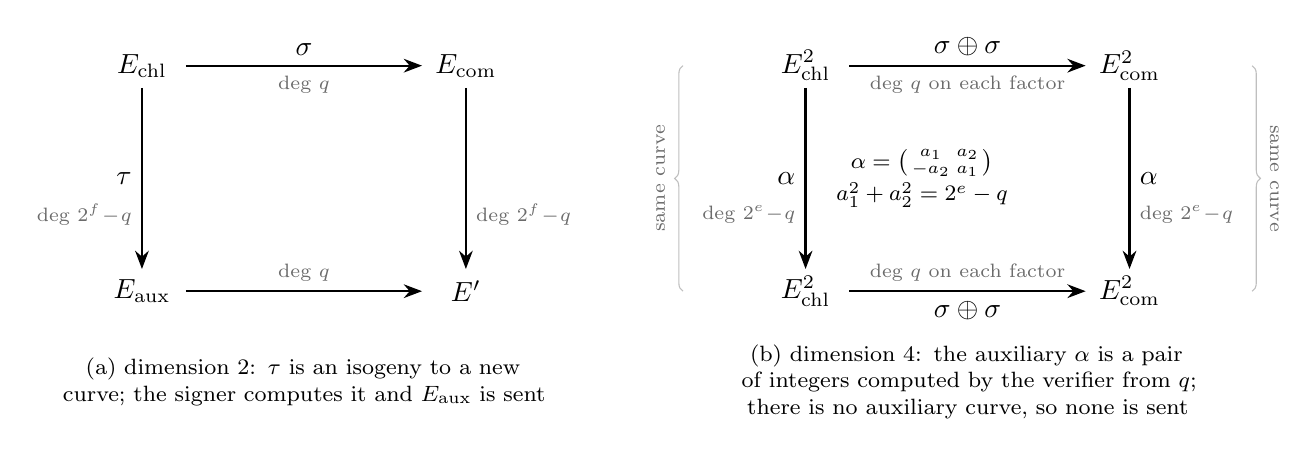
\begin{tikzpicture}
  % ---- (a) dimension 2: the Kani square with its auxiliary corner
  % (the left panel of Figure 1 of the ECLIPSE paper, prism-rs
  % paper/prism-suf/main.tex, with the padlocks removed)
  \node[curve] (Echl) {$\Echl$};
  \node[curve, right=3.0cm of Echl] (Ecom) {$\Ecom$};
  \node[curve, below=2.3cm of Echl] (Eaux) {$\Eaux$};
  \node[curve, below=2.3cm of Ecom] (Ep) {$E'$};
  \draw[->, thick] (Echl) -- node[above] {$\sigma$}
    node[below, deg] {deg $q$} (Ecom);
  \draw[->, thick] (Echl) -- node[left] {$\tau$}
    node[left, deg, pos=0.7] {deg $2^f\!-\!q$} (Eaux);
  \draw[->, thick] (Eaux) -- node[above, deg] {deg $q$} (Ep);
  \draw[->, thick] (Ecom) -- node[right, deg, pos=0.7] {deg $2^f\!-\!q$} (Ep);
  \node[panel, text width=6.4cm] at ($(Eaux)!0.5!(Ep)+(0,-1.15)$)
    {(a) dimension 2: $\tau$ is an isogeny to a new curve; the signer
     computes it and $\Eaux$ is sent};
  % ---- (b) dimension 4: the same Kani square on the doubled curves.  The
  % auxiliary side is the endomorphism alpha, an integer matrix, so the two
  % nodes of each column are one curve and no auxiliary curve exists.
  % Degree labels are the polarized degrees of Kani's lemma, q + (2^e - q)
  % = 2^e, matching panel (a).
  \node[curve, right=3.2cm of Ecom] (Echlt) {$\Echl^2$};
  \node[curve, right=3.0cm of Echlt] (Ecomt) {$\Ecom^2$};
  \node[curve, below=2.3cm of Echlt] (Echlb) {$\Echl^2$};
  \node[curve, below=2.3cm of Ecomt] (Ecomb) {$\Ecom^2$};
  \draw[->, thick] (Echlt) -- node[above] {$\sigma \oplus \sigma$}
    node[below, deg] {deg $q$ on each factor} (Ecomt);
  \draw[->, thick] (Echlt) -- node[left] {$\alpha$}
    node[left, deg, pos=0.7] {deg $2^e\!-\!q$} (Echlb);
  \draw[->, thick] (Ecomt) -- node[right] {$\alpha$}
    node[right, deg, pos=0.7] {deg $2^e\!-\!q$} (Ecomb);
  \draw[->, thick] (Echlb) -- node[above, deg] {deg $q$ on each factor}
    node[below] {$\sigma \oplus \sigma$} (Ecomb);
  % alpha written out beside the left arrow, its sum of squares under it
  \node[anchor=west, align=center, font=\footnotesize, inner sep=1pt]
    at ($(Echlt)!0.5!(Echlb)+(0.35,0)$)
    {$\alpha = \left(\begin{smallmatrix} a_1 & a_2 \\ -a_2 & a_1 \end{smallmatrix}\right)$\\[1pt]
     $a_1^2 + a_2^2 = 2^e - q$};
  % each column of (b) is one curve
  \draw[same] ([xshift=-1.0cm]Echlb.west) -- ([xshift=-1.0cm]Echlt.west)
    node[midway, left=3pt, deg, rotate=90, anchor=south] {same curve};
  \draw[same] ([xshift=1.0cm]Ecomt.east) -- ([xshift=1.0cm]Ecomb.east)
    node[midway, right=3pt, deg, rotate=-90, anchor=south] {same curve};
  \node[panel, text width=7.6cm] at ($(Echlb)!0.5!(Ecomb)+(0,-1.15)$)
    {(b) dimension 4: the auxiliary $\alpha$ is a pair of integers computed
     by the verifier from $q$; there is no auxiliary curve, so none is sent};
\end{tikzpicture}
\caption{The two ways a verifier rebuilds the response; both are Kani
squares.  (a)~In dimension 2 the response $\sigma$ of degree $q$ is
completed by an auxiliary isogeny $\tau$ of degree $2^f - q$ to a new
curve; the signer computes $\tau$ and the signature carries $\Eaux$.
(b)~In dimension 4 the same square sits on the doubled curves and the
complement is the endomorphism $\alpha = \left(\begin{smallmatrix} a_1 &
a_2 \\ -a_2 & a_1 \end{smallmatrix}\right)$ with $a_1^2 + a_2^2 = 2^e -
q$, which the verifier computes from $q$; it acts on $\Echl^2$ and on
$\Ecom^2$ alike, so each column of the square is one curve and there is
no auxiliary curve to send.  The signature carries $\Ecom$, $q$ and the
action of $\sigma$ on the $2^r$-torsion.}
\label{fig:idea}
\end{figure}

\paragraph{Moving the parameters to round 3}
SQIsignHD's exponent $e$ bounds the response degree, $q < 2^e$.  Every
ideal class contains an ideal of norm at most about $0.90 \sqrt{p}$
\cite[Lemma~12]{DLRW24}, so $2^e$ must exceed $\sqrt{p}$, and the paper
takes ``a few bits over $\sqrt{p}$'' as sufficient on a heuristic
(their Section~4.2).
% source: docs/COMPACT_R3.md Section 1, "Theirs".
The library's rule $e = \lambda + \lceil \log_2 2\lambda \rceil$ is
written in the security parameter because at the round-2 primes
$p \approx 2^{2\lambda}$; there it is $\log_2 \sqrt{p}$ plus
$10.8 / 10.0 / 12.6$ bits.  At the round-3 level~I prime, which has 70
bits more than $2^{2\lambda}$, the same formula gives $e = 136$, below the
$2^{162.6}$ that Lemma~12 makes the smallest norm any class is sure to
contain, so no response would exist.  What transfers is the content of
the rule, $\sqrt{p}$ plus about ten bits.
% source: docs/COMPACT_R3.md Section 1, "the SQIsignHD library's rule".

We take $e = \lceil (\log_2 p)/2 \rceil + 11 = \EmbedI / \EmbedIII /
\EmbedV$ and, by the library's own rule for the torsion the two
half-chains need, $r = \lceil e/2 \rceil + 2 = \TorsionRI / \TorsionRIII /
\TorsionRV$ (Table~\ref{tab:parameters}).  The margin of 11 bits is the
library's at the round-2 primes, where its signer found a good $q$ on
every signature; the paper's own prime uses 15.3.  Two checks pin it from
below.  The number of ideal vectors of norm below $2^e$ grows as
$2^{2 \cdot \mathrm{margin}}$, about $2^{22}$ candidates against one good
norm in a few hundred, so a good $q$ exists with overwhelming probability.
And Nakagawa and Onuki's conservative countermeasure for PRISM-id, whose
response reveals an isogeny of large prime degree, is a degree of at least
$4\lambda/3$ bits~\cite[Section~5.3]{NO25}; transferred to $e$, that is
$170.7 / 256.0 / 341.3$ against $\EmbedI / \EmbedIII / \EmbedV$, cleared
at every level, where
8~bits of margin would not clear it at level~I.
% source: docs/COMPACT_R3.md Section 1, "Ours".

\paragraph{The degree}
The signer samples vectors of the response ideal below $2^e$ and keeps the
first whose norm $q$ is odd, congruent to $3$ modulo $4$, and has $2^e -
q$ a probable prime (40 Miller--Rabin rounds).  The verifier repeats the
test on $q$ and decomposes $2^e - q$ by Cornacchia.  The sampled norms
are odd, so one candidate in two passes the congruence; for $2^e - q$
behaving as a random $e$-bit integer the density of good $q$ is then
$1/(e \ln 2)$, one candidate in \ExpectedSamplesOddI{} at level~I, and
\ExpectedTestsI{} candidates per signature reach a primality test.
Section~\ref{sec:bench} measures the loop.
% source: docs/COMPACT_R3.md Section 2 (rule, table and the measured note).

\paragraph{What the verifier checks}
The verifier decodes the key and the signature, recomputes the challenge
from the public key, the commitment curve and the message, completes the
fourth scalar from the pairing relation, tests $q$ for goodness, writes
$2^e - q = a_1^2 + a_2^2$ by Cornacchia, and builds the kernel of the
dimension-4 isogeny on $\Ecom^2 \times \Echl^2$ from $a_1$, $a_2$ and the
transmitted action \cite[Lemma~4 and Section~4.4]{DLRW24}.  It then
computes the two half-chains of $\lceil e/2 \rceil$ steps from both ends
and accepts when the two middle codomains agree and the image of a point
through the chain is what the transmitted action says, the two conditions
of SQIsignHD's Section~4.5.  A signature fails on any decoding error, on a
degree that is not good, on a chain that lands on a product of curves
where it should not, or on either condition.
% source: docs/COMPACT_R3.md Sections 0 and 4 (item 6);
% sqisignhd-harness/round3/README.md.

\paragraph{Whose choices}
SQIsignHD's: the response as an ideal of good norm, the goodness test, the
half-chains of $\lceil e/2 \rceil$ steps from both ends with $r = \lceil
e/2 \rceil + 2$, the transmitted action modulo $2^r$ with the fourth scalar
from the pairing, the verifier's two acceptance conditions (the middle
codomains agree and the image check of their Section~4.5), and the
basis-from-hint convention of their library, kept so that their verifier
can check our signatures unmodified.  Ours: the primes, $e$ and its
margin, the round-3 commitment and its $2^\lambda$ challenge with the
challenge recomputed rather than sent, the wire format with two hint bytes
in place of the library's packed bits, and the signer's sampler, which
draws lattice vectors of the response ideal and rejects on goodness.
% source: docs/COMPACT_R3.md Sections 0, 1, 3 and 4 ("theirs" / "ours").

\begin{table}[H]
\centering
\begin{threeparttable}
\caption{Dimension-4 parameters at the round-3 primes.  Level~I is built
and measured; levels III and V are derived only.}
\label{tab:parameters}
\small
% generated by figures/tab1_parameters.py; do not edit
\begin{tabular}{@{}lccc@{}}
\toprule
 & NIST I & NIST III & NIST V \\
\midrule
$p$\tnote{a} & $3 \cdot 2^{324} - 1$ & $27 \cdot 2^{500} - 1$ & $17 \cdot 2^{664} - 1$ \\
$\log_2 p$\tnote{a} & 325.58 & 504.75 & 668.09 \\
$\lambda$, challenge bits\tnote{a} & 128 & 192 & 256 \\
$e$, response bound $q < 2^e$\tnote{b} & 174 & 264 & 346 \\
$r = \lceil e/2 \rceil + 2$, transmitted torsion bits\tnote{c} & 89 & 134 & 175 \\
half-chain steps $\lceil e/2 \rceil$\tnote{c} & 87 & 132 & 173 \\
\addlinespace
public key, bytes, predicted\tnote{d} & 84 & 130 & 170 \\
signature, bytes, predicted\tnote{d} & 142 & 214 & 280 \\
public key, bytes, measured & 84 & not built & not built \\
signature, bytes, measured & 142 & not built & not built \\
round-3 standard signature, bytes\tnote{a} & 200 & 306 & 406 \\
\bottomrule
\end{tabular}
\begin{tablenotes}\footnotesize
\item[a] The SQIsign round-3 specification \cite{SQISignV3}.
\item[b] Ours: $e = \lceil (\log_2 p)/2 \rceil + 11$ (Section~\ref{sec:dim4}).
\item[c] SQIsignHD's rule for the torsion the half-chains need \cite[Section~4.3]{DLRW24}.
\item[d] Field-by-field sums of the wire format (Section~\ref{sec:dim4}).
\end{tablenotes}

\end{threeparttable}
\end{table}

% ------------------------------------------------------------------------
\section{Benchmarks}
\label{sec:bench}

\paragraph{Method}
One session on one machine, \MachineXeon{} at \XeonGHz{}\,GHz, on
2026-09-26.  One binary measures the Rust code of both rounds: the current
crate for round~3 and the round-2 crate at tag \texttt{v0.4.31} as a
dependency, both compiled by the same \texttt{rustc} in release mode with
fat link-time optimisation and no target-CPU flag.  Each operation is
timed with \texttt{rdtsc} and the wall clock around the call, and the
table reports the median over 50 runs for key generation and signing, 200
for verification, and 100 for the compact signer and verifier.  The C
reference is the-sqisign at tags \texttt{nist-v3} and \texttt{nist-v2},
each built with CMake in \texttt{Release} mode and
\texttt{-DSQISIGN\_BUILD\_TYPE=broadwell}, the assembly-backed field
arithmetic, and measured by its own benchmark
(\texttt{--iterations=300} at level~I, 100 at III and V), medians.  The
round-3 Rust code chooses its assembly field kernels at run time from
CPUID; the round-2 crate has no assembly kernels and signs on a
big-integer library.  Verification is measured from bytes: decode the
key, decode the signature, verify.
% source: paper-dim4/BENCH.md session 2026-09-26 header.

\paragraph{Sizes}
Table~\ref{tab:sizes} lists what the session observed on the wire.  At
level~I the compact key and signature together are \ComboCompactI{} bytes
against \ComboStdI{} for the specification's format, a saving of
\SigSavingPct\,\% on the signature; the compressed dimension-2 format sits
between them at \SigCompI{} bytes.  On the round-2 primes the same three
formats were smaller by the width of the field.
% source: paper-dim4/BENCH.md session 2026-09-26, sizes table.

\begin{table}[H]
\centering
\caption{Public key + signature = total, in bytes, as observed in the
session.  Compact formats are level~I only.}
\label{tab:sizes}
\small
% generated by figures/tab2_sizes.py; do not edit
\begin{tabular}{@{}llccc@{}}
\toprule
primes & format & NIST I & NIST III & NIST V \\
\midrule
round 3 & standard (specification) & 83 + 200 = 283 & 129 + 306 = 435 & 169 + 406 = 575 \\
 & compressed (this crate) & 83 + 176 = 259 & 129 + 269 = 398 & 169 + 353 = 522 \\
 & compact, dim.\ 4 (this crate) & 84 + 142 = 226 & not built & not built \\
\addlinespace
round 2 & standard (specification) & 65 + 148 = 213 & 97 + 224 = 321 & 129 + 292 = 421 \\
 & compact, dim.\ 4 (crate v0.4.31) & 64 + 108 = 172 & not built & not built \\
\bottomrule
\end{tabular}

\end{table}

\paragraph{Cycles}
Table~\ref{tab:bench} is the session in megacycles.  The dimension-4
verifier costs \VerMultI{} times the dimension-2 verifier of the same
crate at level~I; on the round-2 primes the same crate's dimension-4
verifier cost \VerRtwoMultI{} times its dimension-2 one.  Signing in
dimension 4 costs \SignMultI{} times the dimension-2 signer: the good
degree is found by rejection, and the loop is measured in
Table~\ref{tab:loop}.  Key generation is the round-3 key generation in
both formats and differs only in the basis convention
(\KeygenCompactI{} against \KeygenStdI{} megacycles).  The round-3
dimension-2 verifier of the crate runs at \VerStdOverCrefI{} times the
reference's assembly build at level~I, its key generation at
\KeygenStdOverCrefI{} times and its signing at \SignStdOverCrefI{}
times; the compressed format's recovery adds \VerCompOverStdPct\,\% to a
verification.
% source: paper-dim4/BENCH.md session 2026-09-26, Rust and C rows.

\paragraph{The round-2 rows}
The lower half of Table~\ref{tab:bench} is the same two designs on the
round-2 primes, measured in the same session.  The reference's assembly
build verifies a round-2 signature in \VerCrefRtwoI{} megacycles and a
round-3 one in \VerCrefI{}: the price of the primes moved by the 2026
attack, at the same design.  The round-2 crate's dimension-4 verifier cost
\VerRtwoMultI{} times its dimension-2 verifier; on the round-3 prime the
multiple is \VerMultI{}, with half-chains of \HalfStepsI{} steps instead
of 68 on a field of six 64-bit limbs instead of four.  The round-2 crate
has no assembly field kernels and signs on a big-integer library, and its
rows say so.
% source: paper-dim4/BENCH.md session 2026-09-26; docs/COMPACT_R3.md Section 6 (68
% steps, 4-limb field at the round-2 level I prime).

\begin{table}[H]
\centering
\caption{Megacycles, medians of the session.  The last column is the
dimension-4 verifier over the dimension-2 verifier of the same code and
primes.  The C reference is the \texttt{broadwell} build.}
\label{tab:bench}
\small
% generated by figures/tab3_bench.py; do not edit
\begin{tabular}{@{}llrrrc@{}}
\toprule
implementation & level & keygen & sign & verify & $\times$ dim.\ 2 \\
\midrule
\multicolumn{6}{@{}l}{\emph{round-3 primes}} \\
C reference, dimension 2 & I & 35.5 & 101.4 & 11.3 &  \\
C reference, dimension 2 & III & 111.4 & 371.0 & 28.7 &  \\
C reference, dimension 2 & V & 241.5 & 780.6 & 79.8 &  \\
Rust, dimension 2 & I & 39.0 & 113.5 & 12.2 &  \\
Rust, dimension 2 & III & 137.8 & 448.1 & 32.7 &  \\
Rust, dimension 2 & V & 280.1 & 922.6 & 83.0 &  \\
Rust, dimension 2, compressed verify & I & & & 14.4 & \\
Rust, dimension 4 (compact) & I & 41.7 & 336.6 & 120.3 & 9.9 \\
\addlinespace
\multicolumn{6}{@{}l}{\emph{round-2 primes}} \\
C reference, dimension 2 & I & 48.4 & 112.4 & 5.3 &  \\
C reference, dimension 2 & III & 136.9 & 314.4 & 17.0 &  \\
C reference, dimension 2 & V & 210.6 & 527.4 & 32.6 &  \\
Rust, dimension 2 & I & 175.8 & 429.3 & 13.6 &  \\
Rust, dimension 2 & III & 412.2 & 1653.7 & 38.2 &  \\
Rust, dimension 2 & V & 1169.8 & 3036.1 & 77.1 &  \\
Rust, dimension 4 (compact) & I & 173.8 & 204.6 & 108.6 & 8.0 \\
\bottomrule
\end{tabular}

\end{table}

\begin{figure}[htbp]
\centering
\begin{tikzpicture}
\begin{axis}[paperplot, width=9cm, height=5.6cm,
  xlabel={signature bytes}, ylabel={verification, megacycles (median)},
  xmin=120, xmax=240, ymin=0, ymax=140,
  point meta=explicit symbolic, nodes near coords,
  every node near coord/.append style={font=\footnotesize}]
\addplot[only marks, mark=*, mark size=3pt, rsdimtwo,
  every node near coord/.append style={anchor=south west, xshift=3pt, yshift=2pt}]
  table[x=bytes, y=mcyc, meta=format, col sep=comma] {figures/data/fig02_standard.csv};
\addplot[only marks, mark=*, mark size=3pt, rsdimtwo,
  every node near coord/.append style={anchor=south east, xshift=-3pt, yshift=2pt}]
  table[x=bytes, y=mcyc, meta=format, col sep=comma] {figures/data/fig02_compressed.csv};
\addplot[only marks, mark=*, mark size=3pt, rsdimfour,
  every node near coord/.append style={anchor=south west, xshift=3pt, yshift=2pt}]
  table[x=bytes, y=mcyc, meta=format, col sep=comma] {figures/data/fig02_compact.csv};
\end{axis}
\end{tikzpicture}
\caption{The trade at level~I on the round-3 prime: signature bytes
against verification cost for the three formats of one crate, from the
session of Table~\ref{tab:bench}.}
\label{fig:tradeoff}
\end{figure}

\paragraph{Milliseconds}
Table~\ref{tab:ms} gives wall-clock times on two machines for level~I.
Neither machine is what a deployment runs; the ratio between the rows is
the number to carry, and it is the same on both.
% AUTHOR: the M4 Pro column is filled from the author's run of the session
% harness on that machine (paper-dim4/bench, README there); the cells read
% "pending" until paper-dim4/BENCH.md carries the "M4 Pro" table.

\begin{table}[H]
\centering
\caption{Wall-clock milliseconds at level~I, medians.  The M4 Pro column
is pending the author's run on that machine.}
\label{tab:ms}
\small
% generated by figures/tab4_ms.py; do not edit
\begin{tabular}{@{}llrr@{}}
\toprule
format & operation & Xeon, 2.80\,GHz (ms) & M4 Pro (ms) \\
\midrule
round 3, dimension 2 (standard) & key generation & 13.9 & pending \\
 & signing & 40.5 & pending \\
 & verification & 4.4 & pending \\
 & verification, compressed & 5.1 & pending \\
\addlinespace
round 3, dimension 4 (compact) & key generation & 14.9 & pending \\
 & signing & 120.2 & pending \\
 & verification & 43.0 & pending \\
\addlinespace
round 2, dimension 2 (standard) & key generation & 62.8 & pending \\
 & signing & 153.3 & pending \\
 & verification & 4.8 & pending \\
\addlinespace
round 2, dimension 4 (compact) & key generation & 62.1 & pending \\
 & signing & 73.1 & pending \\
 & verification & 38.8 & pending \\
\bottomrule
\end{tabular}

\end{table}

\paragraph{The rejection loop}
Table~\ref{tab:loop} counts the compact signer's search for a good degree
over the session's signatures against the expectation of
Section~\ref{sec:dim4}.  A candidate costs one norm; one in two reaches a
Miller--Rabin test on an $e$-bit number, and composites fail at the first
round.  The spread of signing times in the table is this loop: the median
signature needs \LoopSamplesMedian{} samples, the mean \LoopSamplesMean{},
and the session saw \LoopSamplesMin{} to \LoopSamplesMax{}.
% source: paper-dim4/BENCH.md session 2026-09-26, rejection-loop row and sign rows.

\begin{table}[H]
\centering
\caption{The compact signer's good-degree loop at level~I: measured over
the session's signatures against the density $1/(e \ln 2)$ for odd $q$
(and the figure for a candidate of random parity, which the sampler does
not produce).}
\label{tab:loop}
\small
% generated by figures/tab5_loop.py; do not edit
\begin{tabular}{@{}lrr@{}}
\toprule
 & measured & expected \\
\midrule
signatures measured & 100 & \\
response samples per signature, mean & 114 & 121 \\
\quad the same if $q$ had random parity & & 241 \\
response samples per signature, median (min, max) & 68 (1, 835) & \\
primality tests per signature, mean & 57 & 60 \\
\addlinespace
signing, Mcycles, median (min, max) & 337 (50, 3712) & \\
signing, dimension 2, Mcycles, median & 114 & \\
\bottomrule
\end{tabular}

\end{table}

\paragraph{Memory}
One compact verification at level~I allocates \PeakHeapKiB{} KiB of heap
at its peak (\PeakHeapMiB{} MiB), measured with a counting allocator
around the call; the dimension-2 verifier allocates nothing.
% source: paper-dim4/BENCH.md session 2026-09-26, memory row.

% ------------------------------------------------------------------------
\section{Strong unforgeability, briefly, and ECLIPSE}
\label{sec:suf}

A signature scheme is strongly unforgeable when no one can produce a
second valid signature on a message already signed.  The SQIsign family is
not: in the dimension-2 format the auxiliary isogeny can be replaced by
another of the same degree, giving a second signature that verifies under
the same key.  The round-3 specification states this in its
Section~8.4.2~\cite{SQISignV3}, and the mechanism is written out in
\cite{Ray26}.  Dimension 4 removes the auxiliary curve from the wire but
not the property: a second isogeny of the same degree from the same
commitment curve, with its own action on the torsion, is still a valid
second signature.  This is a property of the scheme, not a finding of
this paper.

A construction that is strongly unforgeable by design exists.  The PRISM
authors describe, next to their salted scheme, a variant whose signature
is one isogeny of prime degree $2^{2e-1} - s^2$ from the public key curve,
and state that the EUF-CMA proof of the salted scheme applies to a salted
version of it~\cite[Section~5 and Remark~11]{PRISMsalt}; we call that
variant \sP{}.  Our instantiation of it on the round-3 primes is named
\ECL{}\footnote{ECLIPSE stands for Encoding-Canonical Large-prime Isogeny
Signature Extension.  The underlying construction, which we call
strong-PRISM, is Section~5 of \cite{PRISMsalt} with the salt of Section~6
as suggested in Remark~11; the authors did not name it.} and is the
subject of a forthcoming paper.

Dimension 4 buys \sP{} nothing.  A PRISM signature carries no auxiliary
curve in any dimension, so there is nothing for dimension 4 to remove; a
dimension-4 instantiation would have the same layout within a few bytes,
and its hash target, a prime $q$ with $2^a - q$ prime and congruent to $1$
modulo $4$, is a second-order prime event, far sparser than the
single-prime target of the dimension-2 variant.  A feasibility study
carried out for prism-rs~\cite{PRISMrs} measured both and declined the
dimension-4 route.

% ------------------------------------------------------------------------
\section{Closing notes}
\label{sec:closing}

\paragraph{Gaps}
One implementation.  There is no independent round-3 dimension-4 signer to
compare against; the SQIsignHD authors' verifier, re-parameterised to our
prime and left otherwise unmodified, accepts our signatures and rejects
tampered ones, which establishes that it agrees with our verifier on our
signer's output and nothing more~\cite{SQISignHDlib}.
% source: docs/COMPACT_R3.md Section 7, step 2 and step 3 to 5 status.
Levels III and V are derived in Table~\ref{tab:parameters} and not built.
Constant time was not attempted for the dimension-4 signer or verifier;
the verifier's integer arithmetic on the degree is variable-time on public
data, and SQIsign signing is variable-time by design in the reference as
well.  The security argument is SQIsignHD's with our parameters
substituted and has not been re-examined; the existence of a good degree
in every class is a heuristic in their paper and stays one here.  The
format is experimental and not for production.

\paragraph{The field}
Three years separate the break of SIDH from a two-dimensional SQIsign in a
NIST round, and one more separates that from primes moved by a new
attack on the isogeny-path problem.  Every construction in this paper is
young, ours included, and the numbers here describe code as it is in
September 2026, not a settled design.  That is the reason for caution in
using any of it.

\paragraph{Thanks}
To the SQIsign authors, Luca De Feo, David Kohel, Antonin Leroux,
Christophe Petit and Benjamin Wesolowski, and the SQIsign2D-West and
round-3 team, for the scheme and the reference code we ported; to the
SQIsignHD authors, Pierrick Dartois, Antonin Leroux, Damien Robert and
Benjamin Wesolowski, for the dimension-4 construction, its library and the
Sage verifier that checks our signatures; and to the PRISM authors,
Andrea Basso, Giacomo Borin, Wouter Castryck, Maria Corte-Real Santos,
Riccardo Invernizzi, Antonin Leroux, Luciano Maino, Frederik Vercauteren
and Benjamin Wesolowski, for the construction that Section~\ref{sec:suf}
names.

\bibliographystyle{alpha}
\bibliography{refs}

\end{document}
